\documentclass[10pt,titlepage]{article}
\usepackage{fullpage}
\usepackage{graphicx}
\usepackage{float}

\begin{document}
  \title{Lab 5: iRobot Hill Climb in C}
  \author{Sam Mansfield and Toan Vuong \\
          TA: Hoekun Kim \\
          EECS149}
  \date{October 9th, 2013}
  \maketitle

  \section{Introduction}
  In this lab we enhanced our previous navigation algorithm to allow the iRobot to navigate up a hill, while remaining aware of and going around obstacles. We made decisions about the priorities of various parts of our algorithm, how often to detect hills, and \textit{what} exactly is a hikk given the robot's sensors.

  \section{Analysis}
    % Describe (and sketch) your climbing algorithm
    Our navigation algorithm remains the same from the last lab. In addition, we also occasionally check for hills by utilizing the myRIO's accelerometer. On an incline, the robot's acceleration in the z-axis will be less than 1g, whereas the magnitude of acceleration in the x and y axes will be more than zero. Using this knowledge, we transition the robot from driving straight to turning when a specific threshold for each accelerometer reading is met. \\ 
    \begin{figure}[H]
        \centering
        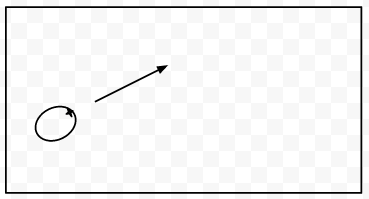
\includegraphics[keepaspectratio,width=0.36\textwidth]{../lab5_data/move.png}
        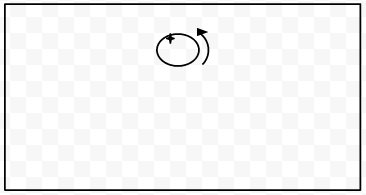
\includegraphics[keepaspectratio,width=0.36\textwidth]{../lab5_data/turn.png}
        \caption{Bird's eye view: The robot making decisions about moving straight vs. turning on a hill.}
    \end{figure}
    The robot will continue to turn until its orientation is forwarding-facing up a hill. To determine the orientation of the robot, we again used accelerometers. Specifically, we know that when the robot is in this orientation, its x-axis reading should be positive, whereas its y-axis reading should be close to zero. This is posited from the way the accelrometers are mounted on the robot. When each sensors are outside of their respective thresholds, we have determined that the robot is now in the correct orientation to continue moving up the hill. \\ 
    \begin{figure}[H]
        \centering
        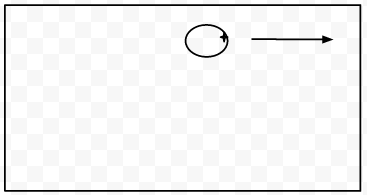
\includegraphics[keepaspectratio,width=0.36\textwidth]{../lab5_data/continue.png}
        \caption{Bird's eye view: The robot resuming an upwards trajectory.}
    \end{figure}
    The last piece of our algorithm involves prioritizing obstacle avoidance versus hill climbing. We merely allowed obstacle avoidance to take precedence over hill climbing: That is, given that a robot is climbing a hill, it will begin its obstacle avoidance algorithm irrespective of which state of the hill climbing algorithm it is in. It will only resume hill climbing once there are no more obstacles. This is a necessary prioritization in order to prevent the robot from falling off a cliff in its quest up the hill.

    % Did you follow a state machine architecture
    To implement this algorithm we followed a state machine architecture without adding any new states from Lab 4. However, we did add additional guards and transitions. 
    \begin{center} 
      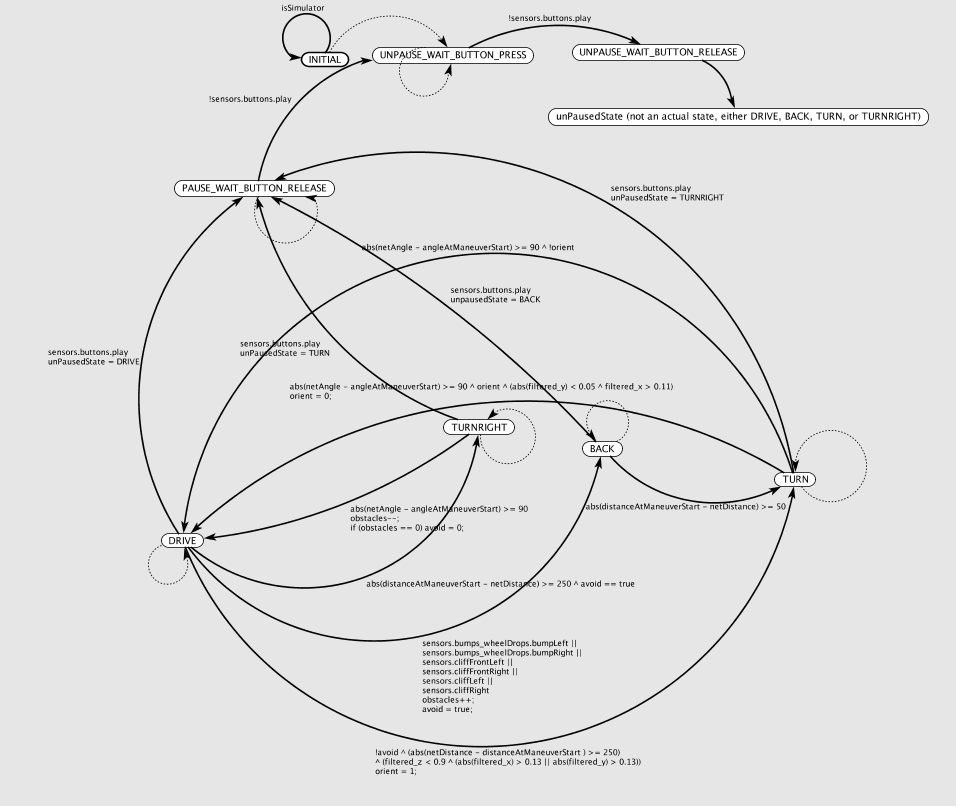
\includegraphics[width=\textwidth]{../lab5_data/FSMLab5}
    \end{center}
    
    % How did you account for movement of the robot when reading from the accelerometer? Describe any algorithms of filters used.
    To account for movement we would only take measurements for tilt after the robot was either in mid drive or mid turn. By doing this the robot should be close to constant velocity and have little effect on the tilt sensing.

    % Feedback
    We had two problems in this lab. One was that we assumed that the accelerometer data being fed to us was already filtered, since in the comments it said it was filtered. After we added our own filter the data was much more stable. Another problem we encountered was that the \texttt{abs()} function only takes integers as arguments. We were feeding in doubles, which did not produce the desired result. We made our own \texttt{absDouble()} function and this improved our algorithm dramatically.

  \section{Conclusion}
    This lab helped us further our use for state machines and also helped us think about how to use accelerometer data effectively. We learned how powerful state machines can be when used properly and how easy it is to change a state machine to add more functionality without having to rewrite the old code, we didn't change our obstacle avoidance state machine at all, only added to it. Learning to use the accelerometer data to sense tilt was very helpful, that way you don't need additional hardware to sense tilt.
\end{document}
